\section{ITK OpenCV Bridge}

\subsection{OpenCV Introduction}

\centeredlargetext{white}{black}{
ITK OpenCV Bridge
}




\begin{frame}
\frametitle{OpenCV Overview}
\begin{center}
\begin{columns}[c]
\column{0.8\textwidth}
\begin{itemize}
\item What is OpenCV?  OpenCV is \ldots
  \begin{itemize}
  \item an open source computer vision library.
  \item written in C, but has C++ and Python APIs.
  \item released under a BSD license.
  \item supported and guided by Willow Garage.
  \item found at \url{http://opencv.willowgarage.com/wiki/}.
  \end{itemize}
\end{itemize}
\column{0.2\textwidth}
 
\includegraphics[width=0.8\textwidth]{../Art/OpenCVLogo.png}
\end{columns}
\pause
\begin{itemize}
\item We will be using OpenCV 2.4 (from subversion).
\end{itemize}
\end{center}
\end{frame}



\begin{frame}
\frametitle{Introduction}
\begin{itemize}
\item ITK Module for working with other libraries
\item Moving frame and/or video data between OpenCV and ITK
\item Bring biomedical and computer vision folks together
\end{itemize}
\end{frame}



\begin{frame}
\frametitle{Design Choices}
\begin{itemize}
\item OpenCV users and ITK users should both be comfortable
\item Image to image utility functions
\item cv::Source to itk::VideoStream
\item Video Group Modules: BridgeOpenCV,BridgeVXL,Core,Filterig,IO
\end{itemize}
\end{frame}

%-------------------------------------------
\subsection{Image Filtering}

\centeredlargetext{white}{black}{
Basic Image Filtering 
itk::image \& cv:mat}

\begin{frame}
\frametitle{Include Header Files}
\framesubtitle{ITKOpenCVBridge/exercise1/BasicFilteringITKOpenCVBridge.cxx}
\begin{itemize}
\item We include ITK and OpenCV headers (like before):
\lstlistingwithnumber{20}{21}{BasicFilteringITKOpenCVBridge.cxx}
\lstlistingwithnumber{23}{24}{BasicFilteringITKOpenCVBridge.cxx}
\item We also need to include the bridge header:
\lstlistingwithnumber{25}{25}{BasicFilteringITKOpenCVBridge.cxx}
\end{itemize}
\end{frame}

\begin{frame}
\frametitle{Basic Layout}
\framesubtitle{ITKOpenCVBridge/exercise1/BasicFilteringITKOpenCVBridge.cxx}
\begin{itemize}
\item The basic layout of this file is the same as the OpenCV
  Examples:
\lstlistingwithnumber{27}{35}{BasicFilteringITKOpenCVBridge.cxx}
\lstlistingwithnumber{69}{84}{BasicFilteringITKOpenCVBridge.cxx}
\end{itemize}
\end{frame}

\begin{frame}
\frametitle{Adding ITK}
\framesubtitle{ITKOpenCVBridge/exercise1/BasicFilteringITKOpenCVBridge.cxx}
\begin{itemize}
\item The type definitions should also be familiar from the ITK
  Material:
\lstlistingwithnumber{38}{45}{BasicFilteringITKOpenCVBridge.cxx}
\item However, notice the bridge class. It contains the conversion function
between OpenCV and ITK.
\lstlistingwithnumber{42}{42}{BasicFilteringITKOpenCVBridge.cxx}
\end{itemize}
\end{frame}

\begin{frame}
\frametitle{From OpenCV to ITK}
\framesubtitle{ITKOpenCVBridge/exercise1/BasicFilteringITKOpenCVBridge.cxx}
\begin{itemize}
\item We call our conversion function to go from a cv::Mat to an
  itk::Image
\lstlistingwithnumber{47}{48}{BasicFilteringITKOpenCVBridge.cxx}
\end{itemize}
\end{frame}

\begin{frame}
\frametitle{Filtering with ITK}
\framesubtitle{ITKOpenCVBridge/exercise1/BasicFilteringITKOpenCVBridge.cxx}
\begin{itemize}
\item The median filtering is normal ITK code, but we do not connect our
output to a writer
\lstlistingwithnumber{49}{64}{BasicFilteringITKOpenCVBridge.cxx}
\pause
\item Instead, we set it to our conversion function
\lstlistingwithnumber{66}{67}{BasicFilteringITKOpenCVBridge.cxx}
\end{itemize}
\end{frame}

\begin{frame}[fragile]
\frametitle{Running the Example}
\framesubtitle{ITKOpenCVBridge/exercise1/BasicFilteringITKOpenCVBridge.cxx}
\begin{itemize}
\item Run the example with the following command
\begin{verbatim}
      ./BasicFilteringITKOpenCVBridge     \
      ~/data/mandrillgray.png             \
      ./mandrillgrayMedian.png            

       eog .mandrillgrayMedian.png
\end{verbatim}
\end{itemize}
\end{frame}

\begin{frame}
\frametitle{Viewing the Results}
\framesubtitle{ITKOpenCVBridge/exercise1/BasicFilteringITKOpenCVBridge.cxx}
\begin{itemize}
\item Running the example the same way as before, we see a nicely
median-filtered image.
\end{itemize}
\begin{columns}[c]
\column{0.33\textwidth}
\begin{center}
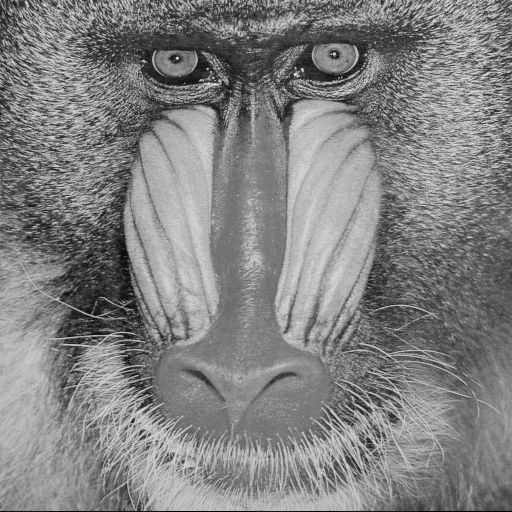
\includegraphics[width=1\textwidth]{../Art/mandrilgray.png} \\
Original
\end{center}
\column{0.33\textwidth}
\begin{center}
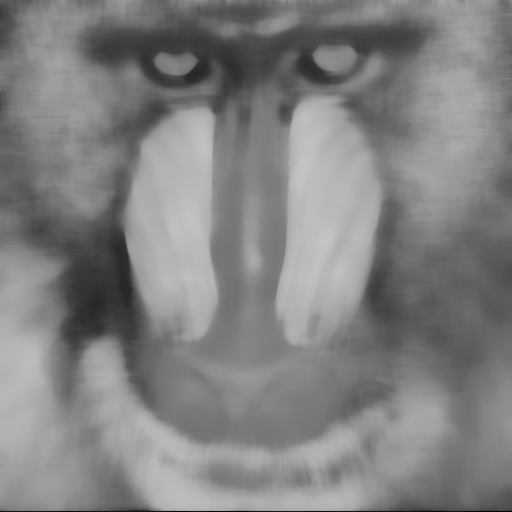
\includegraphics[width=1\textwidth]{../Art/OpenCVITKex1.png} \\
Median Filter
\end{center}
\end{columns}
\pause
\begin{itemize}
\item Now, the fun part. Let's modify our example to use Curvature Flow, an
anisotropic diffusion filter built into ITK.
\end{itemize}
\end{frame}


\begin{frame}
\begin{itemize}
\frametitle{Exercise 1}
\framesubtitle{ITKOpenCVBridge/exercise1/BasicFilteringITKOpenCVBridge.cxx}
\item Hint 1: Curvature Flow requires {\tt float} as the output pixel
  type.
\pause
\item Hint 2: Curvature Flow does not take a radius parameter. It's
  salient functions are:
\lstlistingwithnumber{50}{51}{BasicFilteringITKOpenCVBridgeAnswer.cxx}
\end{itemize}
\end{frame}

\begin{frame}
\begin{itemize}
\frametitle{Exercise 1: Answer}
\framesubtitle{ITKOpenCVBridge/exercise1/BasicFilteringITKOpenCVBridgeAnswer.cxx}
\item First, change the included filter
\lstlistingwithnumber{24}{24}{BasicFilteringITKOpenCVBridgeAnswer.cxx}
\pause
\item The type definitions also need to change to reflect the new
  filter and output image types.
\lstlistingwithnumber{37}{44}{BasicFilteringITKOpenCVBridgeAnswer.cxx}
\end{itemize}
\end{frame}

\begin{frame}
\begin{itemize}
\frametitle{Exercise 1: Answer}
\framesubtitle{ITKOpenCVBridge/exercise1/BasicFilteringITKOpenCVBridgeAnswer.cxx}
\item The semantics of calling the filter also has to change:
\lstlistingwithnumber{50}{51}{BasicFilteringITKOpenCVBridgeAnswer.cxx}
\pause
\item That's it! Now you're using a ``better'' blurring scheme.
\end{itemize}
\end{frame}

\begin{frame}
\begin{itemize}
\frametitle{Exercise 1: Answer}
\framesubtitle{ITKOpenCVBridge/exercise1/BasicFilteringITKOpenCVBridgeAnswer.cxx}
\item The final pipeline should look like this:
\lstlistingwithnumber{35}{35}{BasicFilteringITKOpenCVBridgeAnswer.cxx}
\lstlistingwithnumber{46}{62}{BasicFilteringITKOpenCVBridgeAnswer.cxx}
\end{itemize}
\end{frame}

\begin{frame}[fragile]
\frametitle{Running the Answer}
\framesubtitle{ITKOpenCVBridge/exercise1/BasicFilteringITKOpenCVBridgeAnswer.cxx}
\begin{itemize}
\item Run the answer with the following command
\begin{verbatim}
      ./BasicFilteringITKOpenCVBridgeAnswer     \
      ~/data/mandrillgray.png                   \
      ./mandrillgrayCurvatureFlow.png 
\end{verbatim}
\end{itemize}
\end{frame}

\begin{frame}
\begin{itemize}
\frametitle{Exercise 1: Answer}
\framesubtitle{ITKOpenCVBridge/exercise1/BasicFilteringITKOpenCVBridgeAnswer.cxx}
\item The results should look like this:
\end{itemize}
\begin{columns}[c]
\column{0.33\textwidth}
\begin{center}
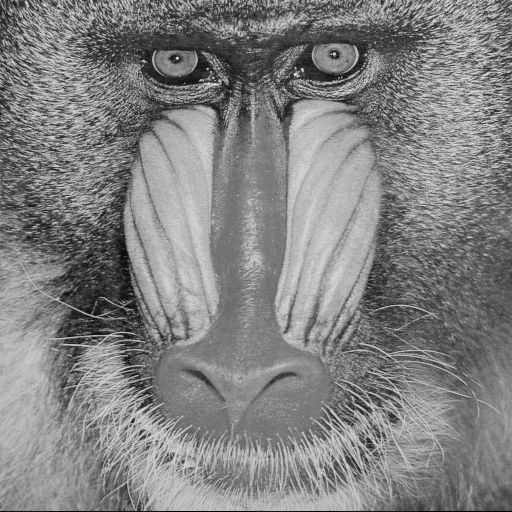
\includegraphics[width=1\textwidth]{../Art/mandrilgray.png} \\
Original
\end{center}
\column{0.33\textwidth}
\begin{center}
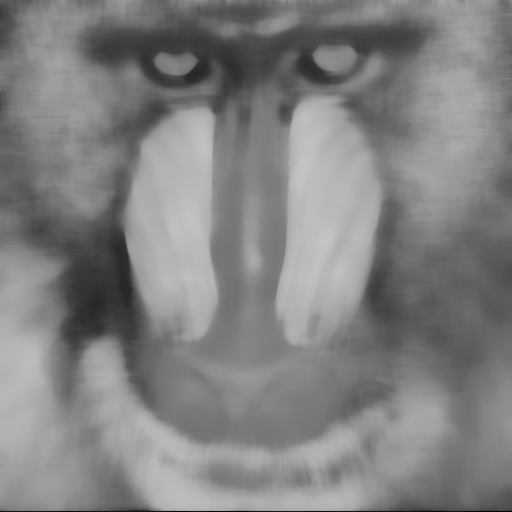
\includegraphics[width=1\textwidth]{../Art/OpenCVITKex1.png} \\
Median Filter
\end{center}
\column{0.33\textwidth}
\begin{center}
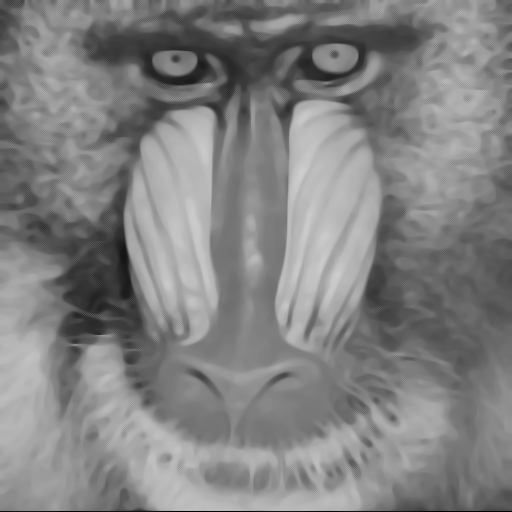
\includegraphics[width=1\textwidth]{../Art/OpenCVITKex1-ans.png} \\
Curvature Flow
\end{center}
\end{columns}
\end{frame}

\subsection{Video Filtering}


\begin{frame}
\frametitle{Basic Video Filtering}
\begin{center}
\begin{itemize}
\item Video filtering is similar to image filtering, except
  \begin{itemize}
  \item use a {\tt VideoCapture} object to read a video file.
  \item loop over each frame in the video and process each one.
  \item display or encode each output frame within the loop.
  \end{itemize}
\end{itemize}
\end{center}
\end{frame}



\begin{frame}
\frametitle{Video Filters}
\begin{itemize}
\item Support video processing natively in ITK
\item Standard framework for multi-frame filters
\item Use ITK's library of image filters in video context
\end{itemize}
\end{frame}


\begin{frame}
\frametitle{More Tutorial Material}
\begin{itemize}
\item  More excercises can be found at:  https://github.com/InsightSoftwareConsortium/ITK-OpenCV-Bridge-Tutorial 
\end{itemize}
\end{frame}




